\documentclass[../thesis.tex]{subfiles}

\begin{document}

\begin{figure}
    \centering
    \begin{subfigure}[b]{0.32\linewidth}
        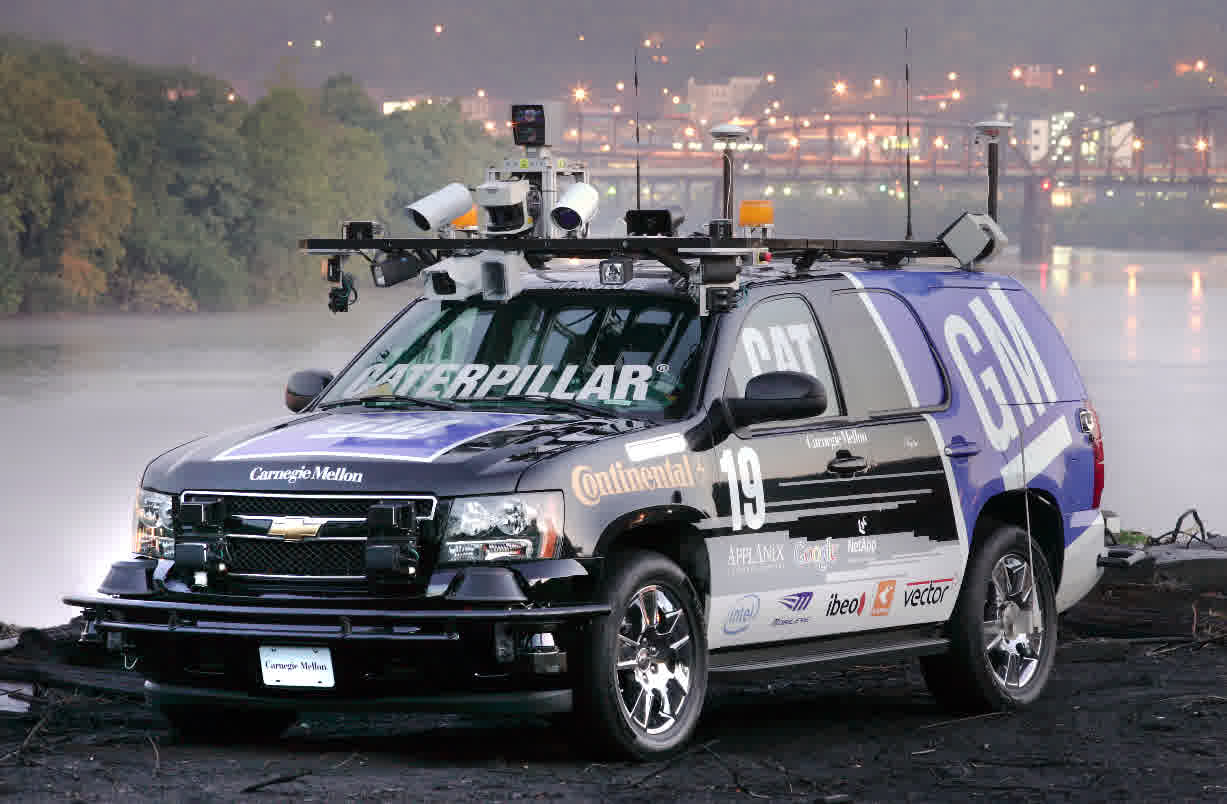
\includegraphics[height=3.5cm]{./Introduction/fig/urban_challenge.jpg}
    \end{subfigure}
    \begin{subfigure}[b]{0.32\linewidth}
        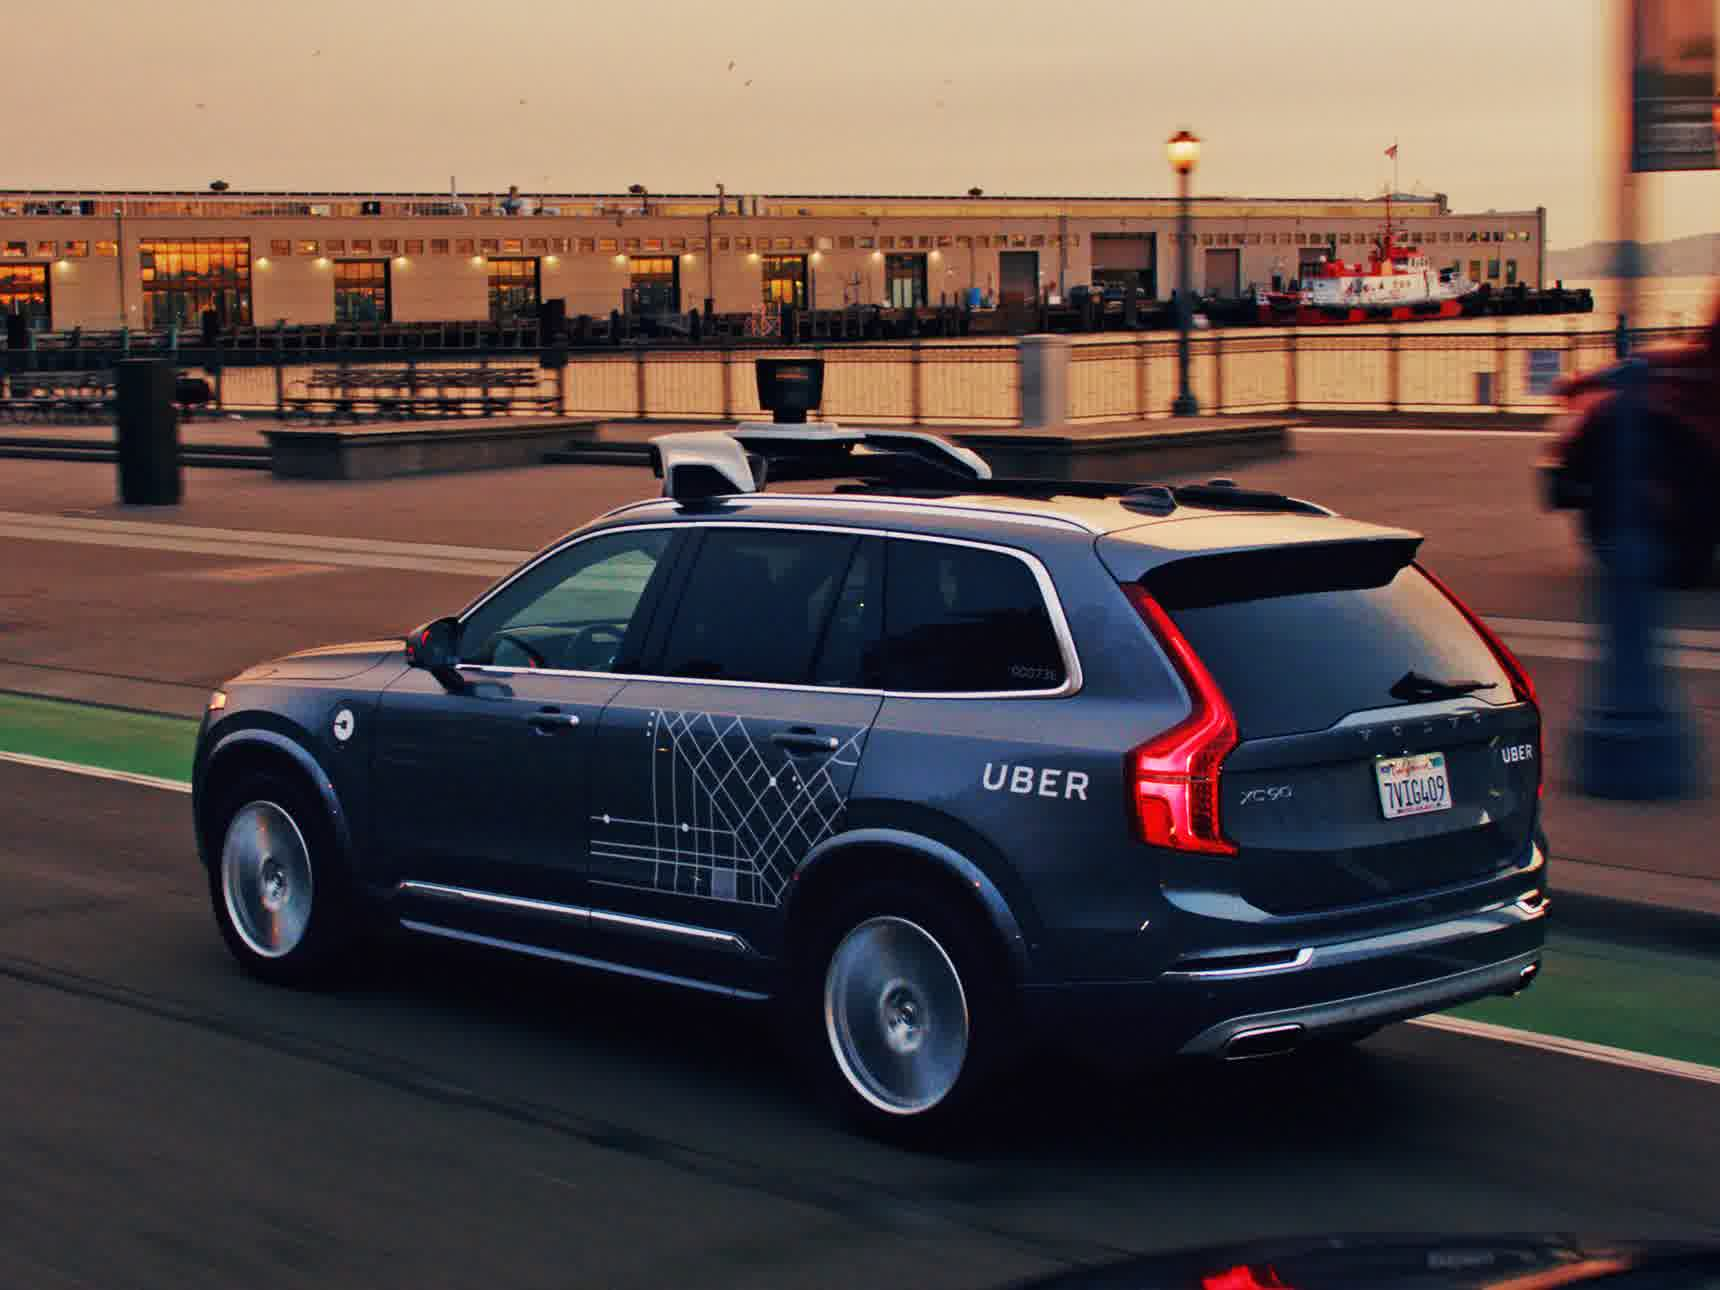
\includegraphics[height=3.5cm]{./Introduction/fig/uber.jpg}
    \end{subfigure}
    \begin{subfigure}[b]{0.32\linewidth}
        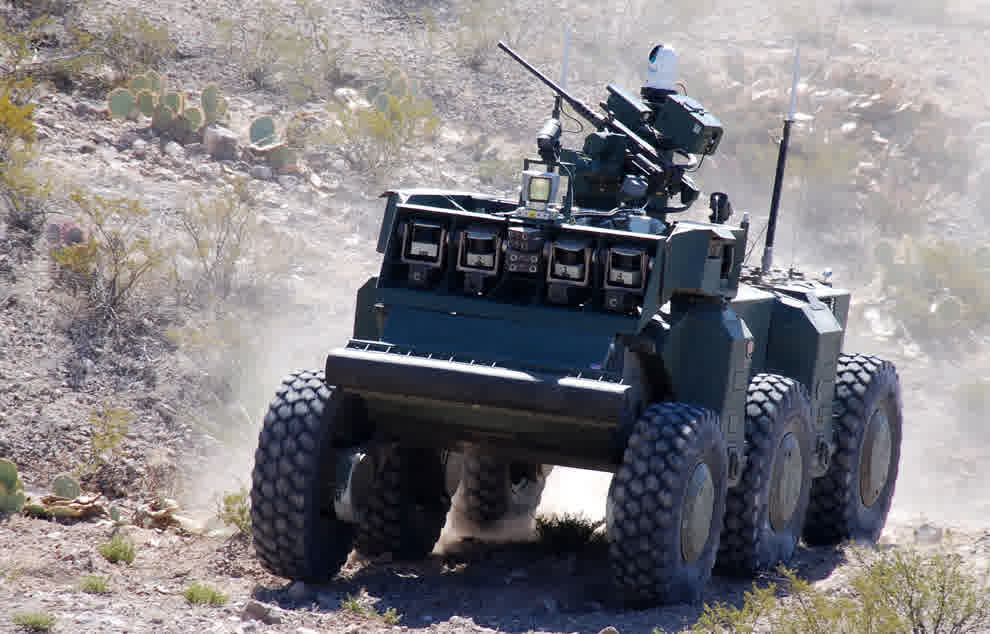
\includegraphics[height=3.5cm]{./Introduction/fig/crusher.jpg}
    \end{subfigure}
    \caption{Some well-known autonomous navigation systems: (a) The Carnegie Mellon Tartan that won the Urban Challenge in 2007 \cite{boss}. (b) Uber's self-driving vehicle. (c) Crusher. \cite{stentz2007crusher}}
    \label{fig:uber_rock}
\end{figure}

\section{Motivation}

%%%  Introduce for on/off-road Autonomous Driving : Motivation %%%

The rapid urbanization globally in the recent past has led to severe road congestion, rise in pollution levels and an increase in road accidents, therefore presenting a very grim picture of the current state of urban transportation. 
At the moment, private automobiles are widely recognized as an unsustainable solution for the future of personal urban mobility \cite{reinventing}. 
Fortunately however, great strides have been made in the development of autonomous driving technologies, energized by the successful demonstrations by some teams at the DARPA Urban Challenge \cite{boss, multimodaltartan}. 
By offering an opportunity to develop sustainable and safe solutions to personal mobility \cite{usecases_of_AD}, they also hint at a complete overhaul of the urban transportation landscape by ushering in Autonomous Vehicles-on-Demand. 
While there is a foreseeable trend on operating autonomous driving technologies on-road within decade, extreme/aggressive motion planning in the off-road situations or unstructured terrains has gained great interests recently \cite{kolter2010probabilistic,williams2016aggressive,gray2012predictive,cutler2016autonomous,cutler2014reinforcement}. 

% Intro to Motion Planning
In modern autonomous systems, \textit{motion planning} refers to a process where a desired movement task is broken into discrete motions that satisfy movement constraints and possibly optimize some aspect of the movement \cite{wiki:motion-planning}. 
For autonomous navigation system, the motion planning algorithm gathers information from sensors, performs optimization over the cost of trajectory toward the desired configuration state (subjected to vehicle constraints if needed), and finally outputs the action commands for execution. 
It is worth noting that for complex decision making tasks, raw sensor information is usually processed through additional \textit{perception} modules to effectively extract informative features before entering the motion planning modules.
In this viewpoint, the motion planning module stands in a crucial position throughout the decision making pipeline in that the potential imperfect sensing, resulted from sensor noise and/or erroneous inference of the perception module, is accumulated here. 
Furthermore, accurate yet efficient decisions need to be made with minimal computations.
This thesis investigates the application of various motion planning approaches in the off-road settings.

\subsection{Traditional Motion Planner}

%%% Intro of Graph base and sample base planner %%%

The two most common approaches for ground vehicles motion planning are graph based planner and sample based planner. 
Both approaches have shown their robustnesses in the DARPA Urban Challenge \cite{koenig2002d,kuwata2008motion} and UPI program \cite{kelly2006toward,stentz2007crusher}, where the feasible trajectories can be solved efficiently under certain reasonable assumptions. The output trajectories can be fine-tuned with optimization techniques to ensure criteria such as smoothness and kinematic constraint \cite{dolgov2008practical}.

%%% Pros and cons of two approach applied to off-road (extreme) navigation %%%

Though graph based planning research has advanced significantly in recent years for the application of off-road navigation \cite{kelly2006toward,stentz2007crusher}, it is limited to the low dimensional configuration space.
For problems that require much more complicated modeling of the dynamic systems, such as maneuvering agilely and aggressively on rough terrain, it will inevitably lead to a higher dimensional configuration space, and thus slows down the standard graph based approaches. 
In fact, one of the main challenges for off-road motion planning comes from the fact that the vehicle dynamics in off-road environment are much more unpredictable in contrast to on-road conditions. 
Factors such as wheel-terrain interaction for modeling the sliding effect is still an active research area \cite{shibly2005equivalent,rubinstein2004detailed}. 
% Maneuvering agilely and aggressively on rough terrain requires a more complex vehicle model, which inevitably leads to a higher dimensional configuration space, and thus slows down the standard graph based approaches. 


Sample based planners on the other hand are more efficient in solving higher-dimensional motion planning. 
Built upon the successful application of randomized approaches to many robotics problems such as manipulation \cite{kuffner2000rrt}, researchers have tried to extend the approach to provide aggressive motion planning for vehicles that exhibit dynamics behaviors such as drifting  \cite{hwan2011anytime}. However, unlike graph based planners that guarantee a certain level of optimality, sample based planner in general only permits asymptotic convergence to the optimal solution. Moreover, it is not straight-forward to implement in kinodynamic problems.

%%% Summary of the traditional motion planner (Link to end-to-end in the next section) %%%

Despite the pros and cons of each approach, they both share a common frameworks where a intelligent pipeline is built to efficiently gather incoming sensor data and take suitable control actions with good repeatability and fault-tolerance. 
The resulting autonomous navigation system is addressed in a modular fashion, where specialized algorithms were developed for each sub-system and finally integrated with some fine tuning.


\subsection{Learning End-to-end Controller}

\begin{figure}[b]
    \centering
    \begin{subfigure}[b]{0.45\linewidth}
        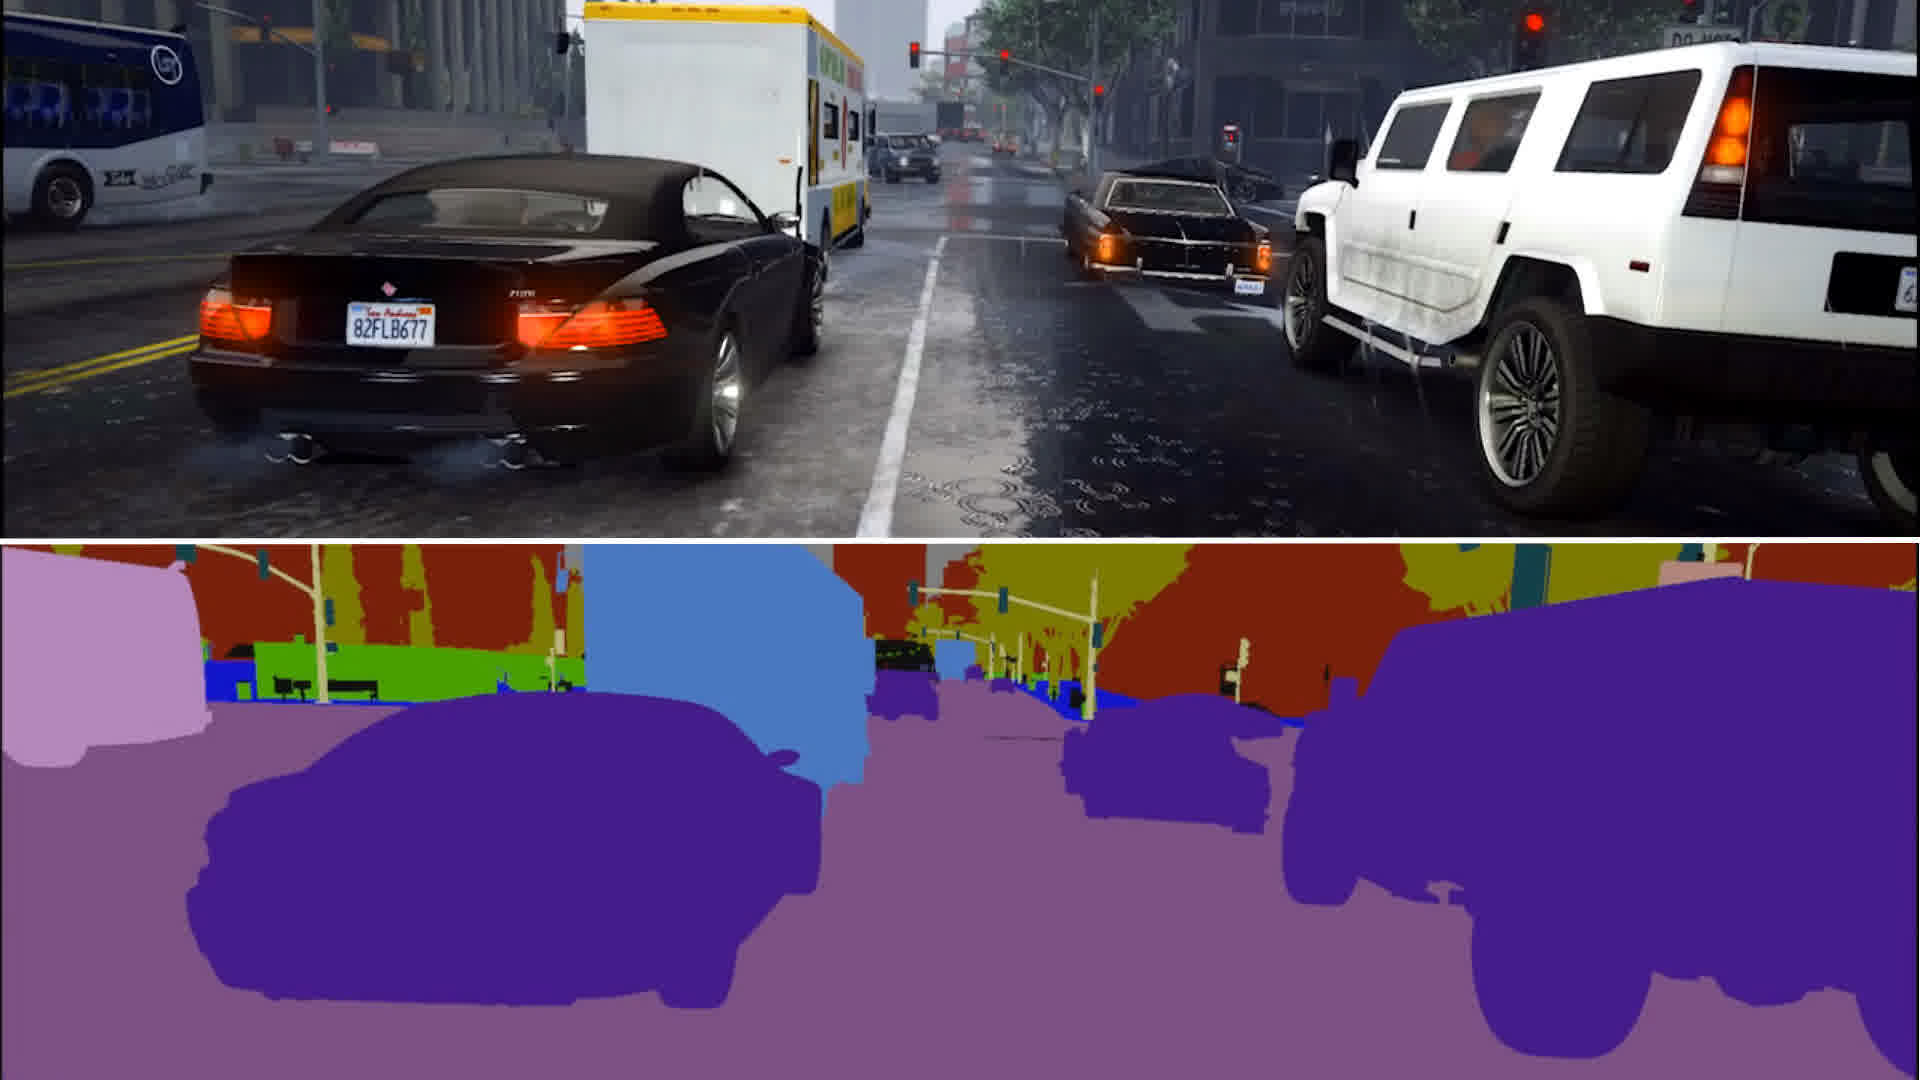
\includegraphics[height=4cm]{./Introduction/fig/gta.jpg}
    \end{subfigure}
    \begin{subfigure}[b]{0.45\linewidth}
        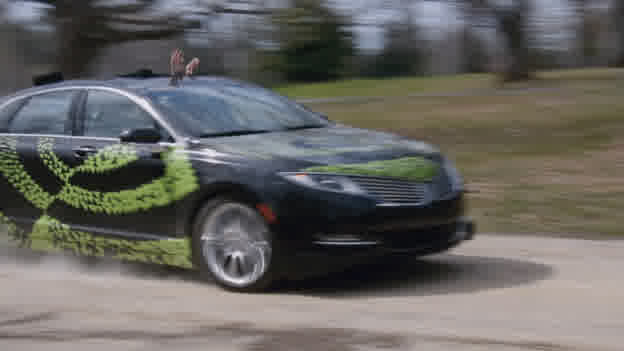
\includegraphics[height=4cm]{./Introduction/fig/nvidia.jpg}
    \end{subfigure}
    \caption{Demonstrations of the end-to-end approach on autonomous navigation applied to (a) the realistic simulator (GTA V), and (b) the full-size vehicle by NVIDIA\cite{nvidiacar}.}
    \label{fig:end-to-end}
\end{figure}

%%% Intro of end-to-end learning  %%%

More recently, however, there is a great interest in applying an end-to-end approach wherein one can learn a complex mapping that goes directly from the input (e.g., camera images or laser scan measurements) to the output (e.g., steering and throttle commands) by leveraging the availability to a large volume of task specific data. 
This approach is purported to perform better since we are optimizing the whole system. 
The end-to-end approaches have become more appealing with the use of deep learning in robotics and has shown successes in developing visuomotor policies for autonomous driving \cite{deepdriving,nvidiacar,endtoendcars}. 
However, the traditional deep supervised learning-based driving requires a great deal of human annotation and may not be able to deal with the problem of accumulating errors \cite{ross2011reduction}. 

%%%  Our choice of using DRL instead of RL  %%%

On the other hand, deep reinforcement learning (DRL) offers a better formulation that allows policy improvement with feedback, and has been shown to achieve human-level performance on several video games \cite{mnih2013playing, mnih2015human,2016-TOG-deepRL}.
The choice of DRL over the more tried and tested waters of Supervised Learning comes from the interest of better generalization and allowing for a more exploration-friendly setting. 
Recently, there have been a great demands and improvements on realistic simulator \cite{deepdrive,udacity} with the hope that the acquired learning in such a simulator can be transferable to the real world with minimal tuning \cite{you2017virtual}. 
% We are inspired by this new development that provides the potential to work around the large sampling requirements of DRL algorithms, and we wish to extend its use to autonomous driving.

%%% Multimodal DRL %%%

Previous work in DRL predominantly learned policies based on a single input modality, \textit{i.e.}, either low-dimensional physical states, or high-dimensional pixels. 
For autonomous driving where enhancing safety and accuracy to the maximum possible extent is top priority, developing policies that operate with multiple inputs is the need of the hour. 
In this light, several recent works in DRL have tried to solve the complex robotics tasks such as human-robot-interaction \cite{qureshi2016robot}, manipulation \cite{levine2016end} and maze navigation \cite{mirowski2017a} with multimodal inputs. 
However, none of the works have explicitly formulated the multimodal sensor policy in terms of sensor fusion, a indispensable technique that improves accuracy and robustness in an autonomous navigation setting. 
This problem is critical as a further step toward the real-world robotics application given the current state-of-the-art DRL agents on many realistic simulators.

In fact, multimodal perception was an integral part of autonomous navigation solutions and even played a critical role in their success \cite{multimodaltartan} before the advent of end-to-end deep learning based approaches. 
It offers several advantages, namely robustness to individual sensor noise/failure, improved object classification and tracking \cite{elfring2016multisensor, cho2014multi, darms2008classification}, robustness to varying weather and environmental conditions, etc. 
It is worth mentioning that though \citet{mirowski2017a} uses multimodal sensors to navigate through a maze, information such as depth is only used as an auxiliary loss, \textit{i.e.} it is not an input to the trained policy but is only used to improve the learning outcomes. 
In fact, \citet{mirowski2017a} pointed out that the naive RGBD policy performs worse than predicting depth as a regression task,


\begin{figure}[b]
	\vskip -0.1in
    \centering
    \begin{subfigure}[b]{0.45\linewidth}
        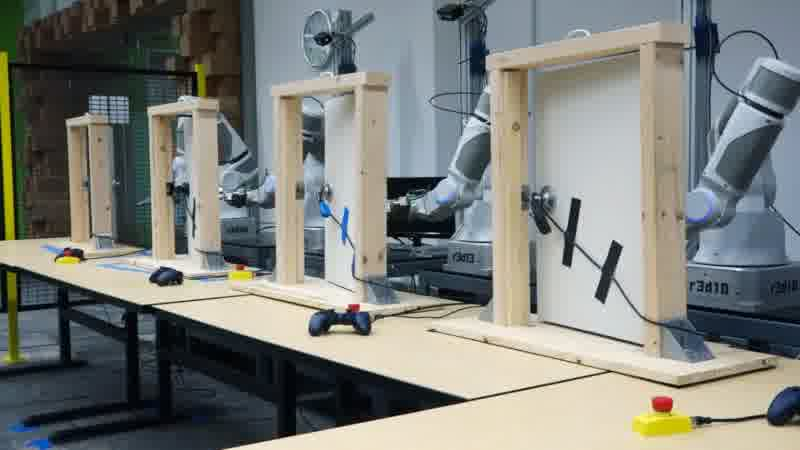
\includegraphics[height=3.5cm]{./Introduction/fig/drl_manipulation.jpg}
    \end{subfigure}
    \begin{subfigure}[b]{0.45\linewidth}
        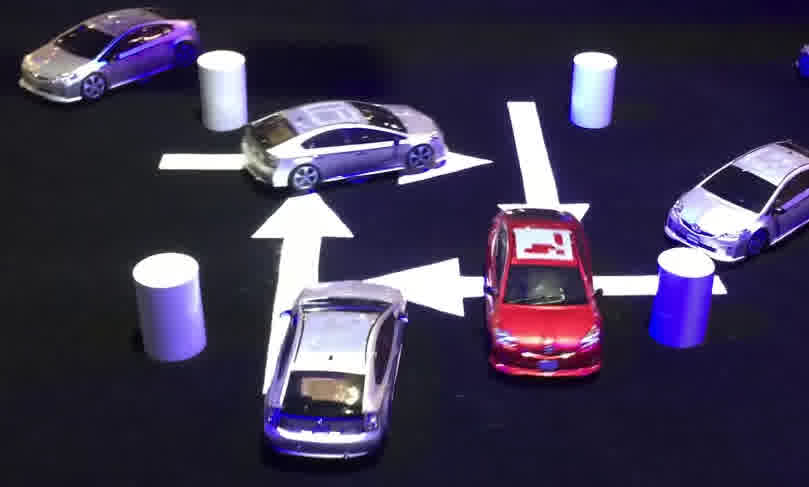
\includegraphics[height=3.5cm]{./Introduction/fig/drl_perfer_network.jpg}
    \end{subfigure}
    \caption{Recent successes on applying deep reinforcement learning (DRL) algorithms to real-world robotics problems: (a) manipulation \cite{gu2016deep}. (b) autonomous navigation. \cite{prefernetwork}}
    \label{fig:end-to-end}
\end{figure}


\section{Approaches}

In this work, we first propose a model-based local planner solve the optimal kinodynamic motion planning problem. 
The local planner is built upon a vehicle model that effectively captures important state for off-road navigation such as lateral velocity. 
Practical problems such as re-planning and optimization are addressed under the standard sample based approach, but modified appropriately to encourage a more aggressive maneuvering. 
The resulting model-predictive planner was tested on the full-size All-Terrain Vehicle (ATV) in the off-road conditions.

We also present an alternative end-to-end controller that uses multi-sensor input to learn an autonomous navigation policy in a physics-based gaming environment called TORCS \cite{wymann2000torcs}. 
To show the effectiveness of multimodal perception, we pick two popular continuous action DRL algorithms namely Normalized Advantage Function (NAF) \cite{CDQN} and Deep Deterministic Policy Gradient (DDPG) \cite{DBLP:journals/corr/LillicrapHPHETS15}, and augment them to accept multimodal inputs. 
Though a multimodal sensor policy may greatly improve the reward, it might rely heavily on all the inputs to the extent that it may fail completely even if a single sensor broke down fully or partially. This undesirable consequence renders sensor redundancy useless. 
To ensure that the learned policy does not succumb to such over-fitting, we apply a novel stochastic regularization method called \emph{Sensor Dropout} during training. 
Our approach reduces the policy sensitivity to a particular sensor subset, and makes it capable of functioning even in the face of partial sensor failure. 
Based on the Sensor Dropout, we further embedded the standard DRL loss with an auxiliary loss that help reduce the action variations of the multimodal policy. 
As far as we know, we are the first to address the multimodal policy learning in terms of sensor fusion.

Through empirical testing we demonstrate that our proposed multimodal sensor policy can 1) operate with minimal performance drop in noisy environments, and 2) remain functional even in the face of a sensor subset failure. 
Finally, through the visualization of gradients, we show that the learned policies are conditioned on the same latent input distribution despite having multiple sensory observations spaces - a hallmark of true sensor-fusion.
Suitable metrics have been devised to study this behavior and highlight its applicability to other domains.

Note that both the traditional and the end-to-end planner require the cost/reward heuristic function to guild the policy and formally define the optimization problem. 
However, unlike in the urban environment where cost function can be well defined in a rule-based structure, finding a cost function for off-road navigation can be nontrivial and often requires lots of handy tuning. \cite{silver2010learning}
Here, motivated by the recent successes \cite{wulfmeier2015maximum,wulfmeier2016watch}, we also investigate into the using deep neural network as the function approximator, and infer the cost/reward function under inverse reinforcement learning (IRL) platform. 
Again, we can leverage the availability to a large volume of task specific data and solve the problem with minimal engineering hand-tuning.

% TODO
To summarize, the primary contributions of this thesis are:
\begin{enumerate}

    \item %RRT
    Propose a model-based local planner for high-speed maneuvering in the off-road navigation application. 
    The planner uses Rapidly-exploring Random Tree (RRT) \cite{kuffner2000rrt} as its template, and is tested on a full-size all-terrain vehicle (ATV) in the off-road environment. 
    We show that the planner is capable of performing smooth yet aggressive avoid static obstacles with high speed up to $30 kph$.

    \item % M-DRL
    Propose a new stochastic regularization, namely \emph{Sensor Dropout}, for training an end-to-end multi-sensor policy under deep reinforcement learning (DRL) framework. 
    The proposed method is integrated with two popular continuous action algorithms and heavily tested on a physics-based gaming environment called TORCS \cite{wymann2000torcs}. 
    We show that policies trained with Sensor Dropout not only perform minimal performance drop when measurements become noisy/imperfect, but are also less sensitive to any single sensing modality; therefore makes it able to function even in the face of partial sensor failure.

    \item % DIRL
    Investigate into the deep inverse reinforcement learning (DIRL) algorithms that infer the cost, or traversibility, of the unstructured terrain by leveraging large volume of human demonstration data collected on field. 
    We propose two slight modifications over the current approach \cite{wulfmeier2015maximum}, including explicitly modeling the ambiguity of optimality, and integrating with failure demonstrations to overcome the spatially sparse gradient of DIRL.
    The framework is tested on a full-size all-terrain vehicle (ATV) in the off-road environment.

\end{enumerate}

The thesis is organized as follows:
In Chapter \ref{chap:related_work} we briefly go through the preliminary background, including the basic sample based planner, the formal definition of deep (inverse) reinforcement learning, and the two continuous action agents used in this work.
In Chapter \ref{chap:rrtplanner} we formulate our model predictive planner, followed with the derivation of vehicle model, detailed planner design for optimal planning, and finally the experimental results on field.
In Chapter \ref{chap:multimodalDRL} we propose a new technique at the aspect of sensor fusion in order to improve the performance of the end-to-end controller with multi-sensor inputs. 
In Chapter \ref{chap:dirl} we investigate the traversibility analysis with the recently popular studies on deep inverse reinforcement learning.
Finally, we conclude the work in \ref{chap:conclusion} and address some of the interesting direction for future works.

\end{document}
